

% ****** Start of file aipsamp.tex ****m*
%
%   This file is part of the AIP files in the AIP distribution for REVTeX 4.
%   Version 4.1 of REVTeX, October 2009
%
%   Copyright (c) 2009 American Institute of Physics.
%
%   See the AIP README file for restrictions and more information.
%
% TeX'ing this file requires that you have AMS-LaTeX 2.0 installed
% as well as the rest of the prerequisites for REVTeX 4.1
% 
% It also requires running BibTeX. The commands are as follows:
%
%  1)  latex  aipsamp
%  2)  bibtex aipsamp
%  3)  latex  aipsamp
%  4)  latex  aipsamp
%
% Use this file as a source of example code for your aip document.
% Use the file aiptemplate.tex as a template for your document.
\documentclass[%
 aps, prl,
% jmp,
% bmf,
% sd,
% rsi,
 amsmath,amssymb,
%preprint,%
 reprint,%
%author-year,%
%author-numerical,%
% Conference Proceedings
superscriptaddress
]{revtex4-2}

\usepackage{graphicx}% Include figure files
%\usepackage{dcolumn}% Align table columns on decimal point
\usepackage{bm}% bold math
\usepackage{fixme}
%\usepackage[mathlines]{lineno}% Enable numbering of text and display math
%\linenumbers\relax % Commence numbering lines
\usepackage{hyperref}
\usepackage{kbordermatrix}% http://www.hss.caltech.edu/~kcb/TeX/kbordermatrix.sty
\usepackage[utf8]{inputenc}
\usepackage[T1]{fontenc}
\usepackage{mathptmx}
\usepackage{lipsum}
\usepackage{amsmath}
\usepackage{physics}
\usepackage{xparse}
\usepackage{bbm}
\usepackage{xcolor}
\usepackage{url}


%\usepackage{multirow}
%\usepackage{makecell}
\graphicspath{{Pictures/}}

\renewcommand*{\figureautorefname}{Fig.}
\renewcommand*{\equationautorefname}{Eq.}

\newcommand{\mytitile}{Photon transport in a Bose-Hubbard chain of superconducting artificial atoms}

\begin{document}
	\preprint{AIP/123-QED}
	
	\title[\mytitile]{\mytitile\\~}
	\author{G.P. Fedorov}
	\email{gleb.fedorov@phystech.edu}
	
	\affiliation{ 
		Russian Quantum Center, National University of Science and Technology MISIS, 119049 Moscow, Russia
	}%
	\affiliation{ 
		Moscow Institute of Physics and Technology, Dolgoprundiy, Russia
	}
	\author{S. Remizov}
	\affiliation{Dukhov Automatics Research 
		Institute, (VNIIA), Moscow, Russia}
	\author{V. Pogosov}
	\affiliation{Dukhov Automatics Research 
	Institute, (VNIIA), Moscow, Russia}
	\author{D. Shapiro}
	\affiliation{Dukhov Automatics Research 
	Institute, (VNIIA), Moscow, Russia}

	\author{I.A. Rodionov}
	\affiliation{FMN Laboratory, Bauman Moscow 
		State Technical University, Moscow, Russia}
	\affiliation{Dukhov Automatics Research 
	Institute, (VNIIA), Moscow, Russia}

	\author{O.V. Astafiev}
	\affiliation{Skolkovo Institute of Science 
		and Technology, Moscow, Russian Federation}
	\affiliation{ 
		Moscow Institute of Physics and Technology, 
		Dolgoprundiy, Russia
	}
	\affiliation{Physics Department, Royal 
	Holloway, University of London, Egham, Surrey 
	TW20 0EX, United Kingdom}
\affiliation{National Physical Laboratory, Teddington, TW11 0LW, United Kingdom}

	\author{A.V. Ustinov}
	\affiliation{ 
		Russian Quantum Center, National University of Science and Technology MISIS, 119049 Moscow, Russia
	}
	\affiliation{Physikalisches Institut, Karlsruhe Institute of Technology, 76131 Karlsruhe, Germany}
	
	
	\date{\today}% It is always \today, today,
	%  but any date may be explicitly specified
	
	
	\begin{abstract}
We investigate non-equilibrium steady-state photon transport through a chain of five coupled artificial atoms described by the Bose-Hubbard model. The system retains many-particle coherence while still being coupled strongly to the open spaces. We show that system energy bands may be visualized with high contrast using cross-Kerr interaction. For vanishing disorder, we demonstrate transport in linear and nonlinear regime of photon blockade and show excellent agreement of with the input-output theory for a model including around a hundred basis states. Finally, we show how controllable disorder in the system suppresses this non-local photon transmission. We argue that suggested architecture may be applied to analog simulation of many-body Floquet dynamics with even larger arrays of artificial atoms paving an alternative way to demonstration of quantum supremacy.
\end{abstract}
	
\maketitle



There has been increased effort over recent years in on-chip simulation of various solid state and quantum optical models using superconducting circuits \cite{kjaergaard2019superconducting}. The Bose-Hubbard (B-H) model is now particularly well-covered as it can be straightforwardly mapped onto arrays of coupled transmon qubits \cite{orell2019probing,yanay2020two}. The pioneering work \cite{hacohen2015cooling} had demonstrated this for a three-site linear lattice, and subsequent experiments were focused on simulating dynamics with engineered dissipation \cite{ma2019dissipatively}, investigating the many-body localization phase transitions \cite{roushan2017spectroscopic,chiaro2019growth}, and correlated quantum walks \cite{Yan2019, Ye2019}. As numerous theoretical studies propose a new research direction involving controllable light-matter interaction and Floquet engineering to study periodically-driven Hamiltonians and their non-equilibrium dynamics \cite{Goldman2014, eisert2015quantum, Zippilli2015, kyriienko2018floquet, franca2020simulating}, it is tempting to use transmon chains  to simulate the driven-dissipative Bose-Hubbard model. The subject is particularly interesting since a recent study has shown that driven systems may open new ways to demonstrate quantum supremacy \cite{tangpanitanon2019quantum}.

In this Letter, we present a proof-of-principle device which models non-equilibrium steady-state boson transport through a Bose-Hubbard chain using a linear array of five transmons strongly coupled to waveguides at its edges. This strong coupling, however, being much smaller than the interaction between the transmons does not destroy the many-body coherence of the system. Our results thus imply that such architecture with an increased number of transmons could be suitable for supremacy-scale Floquet quantum simulations. Moreover, this device complements previous theoretical research on the transmission spectroscopy of quantum metamaterials \cite{Zagoskin2016, viehmann2013observing, Greenberg2015, Fistul2019, Biella2015,roberts2020driven, collodo2019observation} with direct experimental data. We also expect that these systems may be used to test the accuracy of methods of contraction of the Hilbert space such as the matrix product states or tensor networks in general \cite{Biella2015, orell2019probing, di2019efficient}.

The layout of the chip is shown in \autoref{fig:scheme}~(a). We use a chain of capacitively coupled Xmon qubits tunable via individual flux lines. Physically, strong coupling is attained via large interdigitated capacitors at the input and output waveguides and allows to measure the microwave transmission through the system. In \autoref{fig:scheme}~(b), we illustrate the physical model that simulated by the device; the corresponding Hamiltonian including the coherent drive is
\begin{equation}
\begin{aligned}
\hat H/\hbar &= \sum_{i=1}^5\left[ (\omega_i - \omega_d) \hat b^\dag_i \hat b_i + \frac{1}{2} \alpha_i \hat b_i^\dag \hat b_i (\hat b^\dag_i \hat b_i - 1)\right]\\
&+\sum_{i=1}^4 J (\hat b^\dag_{i+1} \hat b_i + \hat b_{i+1} \hat b_i^\dag)+\frac{\Omega}{2}(\hat b_1^\dag + \hat b_1),
\end{aligned}\label{eq:bose-hubbard}
\end{equation} 
where $\hat b_i$, $\hbar \omega_i$ and $\hbar\alpha_i$ are, respectively, site lowering operator, single-boson energy, on-site interaction for the $i$\textsuperscript{th} site; $J$ is the site-site tunneling rate, and $\omega_d$ is the drive frequency \cite{egorova2020analog, PhysRevA.102.013707, yanay2020two}. The dissipation in the system is essential for the dynamics as it mostly comes from the waveguides and is included in the corresponding Liouville equation using Lindbladian superoperators $\mathcal D[\hat{O}^{(i)}_\alpha] = \hat{O}^{(i)}_\alpha \hat \rho \hat{O}^{(i)\dag}_\alpha - \frac{1}{2}\{\hat{O}^{(i)\dag}_\alpha \hat{O}^{(i)}_\alpha, \hat \rho\},$ where $\hat{O}^{(i)}_\gamma = \sqrt{\gamma_i} \hat b_i$ is the relaxation and $\hat{O}^{(i)}_\phi = \sqrt{\gamma^{(i)}_\phi} \hat b_i^\dag \hat b_i$ is the pure dephasing. Strong coupling to the edge lines implies $\gamma_1 \approx \gamma_5 \approx \Gamma$ to be the dominating source of decoherence. If $\omega_i = \omega,\ \alpha_i = \alpha$, the standard Bose-Hubbard Hamiltonian is restored.


\begin{figure}
	\centering
	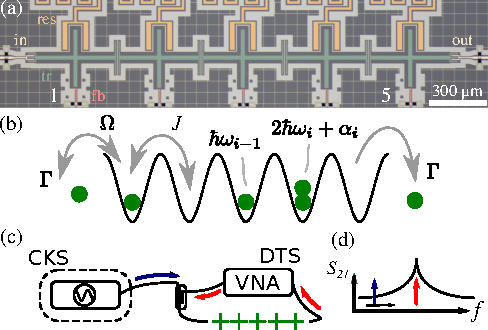
\includegraphics[width=1\linewidth]{Pictures/scheme.pdf}
	\caption{\textbf{(a)} Optical image of the device (false-colored). Input and output waveguides (beige) are strongly coupled to the edge transmons (green). All transmons can be dispersively read out via auxiliary resonators (orange) and tuned via flux bias lines (red). \textbf{(b)} Model of the device as a B-H lattice with five sites. Bosons are inserted from the left by a drive of strength $\Omega$, and can leak from both sides at rate $\Gamma$. The energy of an i\textsuperscript{{th}} localized boson is $\hbar \omega_i$, and adding another boson to the same site costs $\hbar \alpha_i < 0$. Bosons can tunnel between sites at rate $J$. \textbf{(c)} Qualitative measurement scheme: the direct transmission spectroscopy (DTS) is done using the vector network analyzer which measures the complex transmission $ S_{21} $. The cross-Kerr spectroscopy (CKS) requires an additional microwave source. \textbf{(d)} The CKS is done by sweeping the source frequency (blue arrow) while monitoring the transmission amplitude at some resonance peak via the VNA (red arrow).}
	\label{fig:scheme}
\end{figure}
	

In \autoref{fig:scheme}~(c) we show schematically the experimental setup. We measure the transmission $S_{21}$ through the chain using a vector network analyzer (direct transmission spectroscopy, DTS), and optionally use an additional microwave source to perform the cross-Kerr spectroscopy (CKS) of the system. With the continuous microwave excitation, we study the steady-state properties of the device. To obtain theoretical predictions for the $S_{21}$ in the steady state, one can use the input-output formalism \cite{yurke1984quantum,gardiner1985input}. Since we irradiate the system coherently, we assume that the input field mode amplitude is related to the coherent drive strength $\Omega$ in the driving operator $\hbar \Omega \hat b_1 \cos \omega t$ via $\sqrt{\gamma_1} \langle  \hat b_{in}^\dag \rangle \approx i \Omega/2$, which follows from the quantum Langevin equations when disregarding the noise term. Similarly, the output field operator $\hat b_{out}^\dag \approx \sqrt{\gamma_5} \hat b_5^\dag$. From this, we obtain $
	S_{21} = \langle \hat b_{out}^\dag\rangle / \langle \hat b_{in}^\dag \rangle = 2\Gamma\cdot \Tr[\hat \rho_{ss} \hat b_5^\dag]/{i\Omega} ,
$,
where $\hat \rho_{ss}$ is the steadystate density matrix. Physically, this expression means that the signal transmission would be possible if the rightmost transmon becomes non-locally excited while the leftmost one is subject to radiation. From the Langevin equations follows that in the limit of $\Omega \ll \Gamma$, the system can be linearized \cite{astafiev2010resonance}. At the degeneracy point ($\omega_i = \omega$), five transmission peaks appear at $0,\, \pm J,\, \pm \sqrt{3} J$ from $\omega$ due to the strong interaction, corresponding to the classical normal mode frequencies. The widths of the central, next-to-central and edge peaks are $2\Gamma/3,\ \Gamma/2$ and $\Gamma/6$, respectively, and add up to $2\Gamma$ (see Supplements).  In the quantum-mechanical limit, these resonances should remain in the spectrum due to the correspondence principle; however, new lines caused by purely quantum-mechanical processes are expected to appear in the nonlinear regime.

\begin{figure}[b]
	\centering
	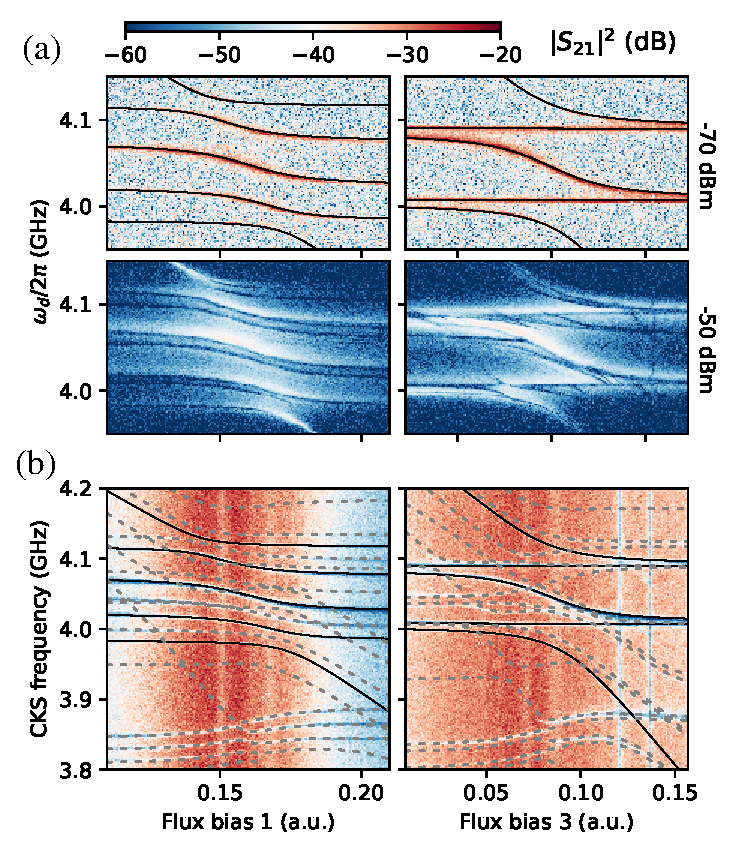
\includegraphics[width=1\linewidth]{Pictures/fig2}
	
	\caption{\textbf{(a)} DTS of the chain. $S_{21}$ includes the attenuation and amplification in the measurement chain, VNA output power is shown on the right. In the top row, black lines are the fit of the lowest five transitions of \autoref{eq:bose-hubbard} for $J/2\pi = 41$ MHz, $\omega_i/2\pi \approx 4.05$ GHz. \textbf{(b)} CKS via the the third mode showing the emergent band structure of the system. Dashed lines are fits to the purely quantum transitions.}
	\label{fig:transmission}
\end{figure}



\begin{figure*}
	\centering
	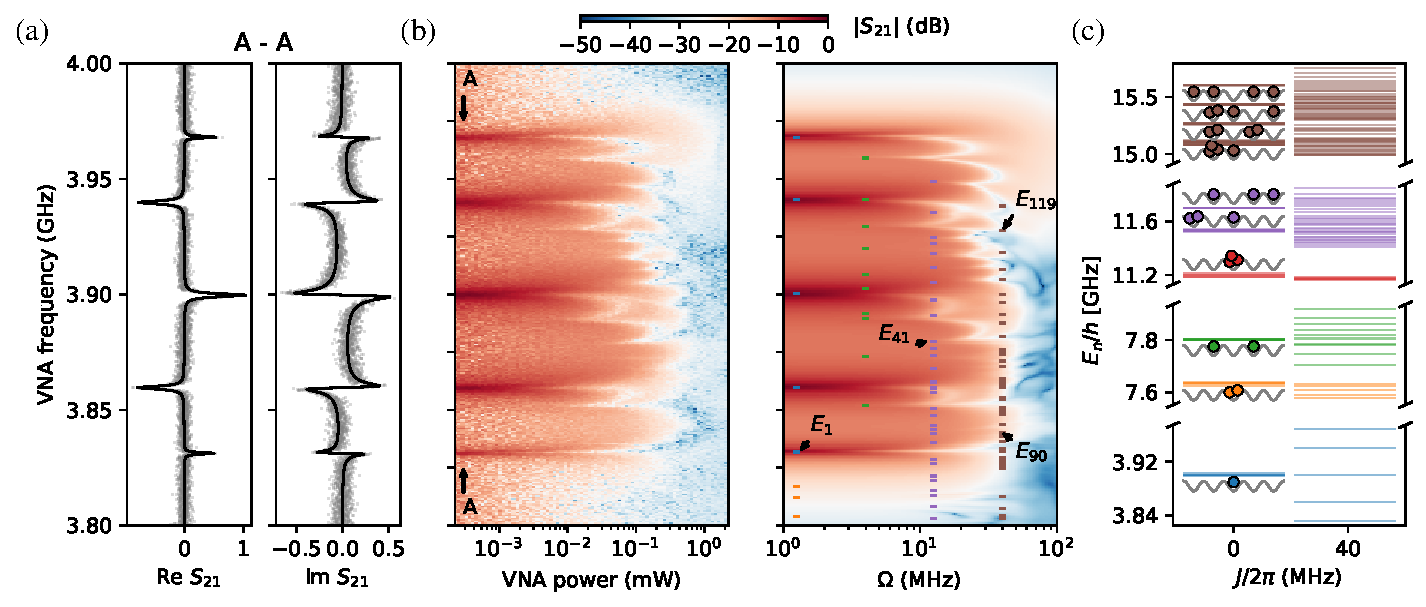
\includegraphics[width=\linewidth]{Pictures/fig3}
	
	
	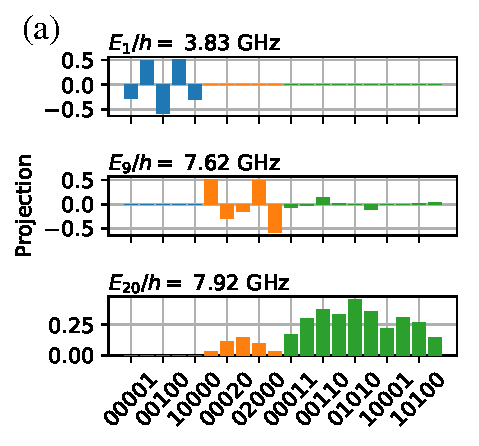
\includegraphics[width=.33\linewidth]{Pictures/eigenstates1}
	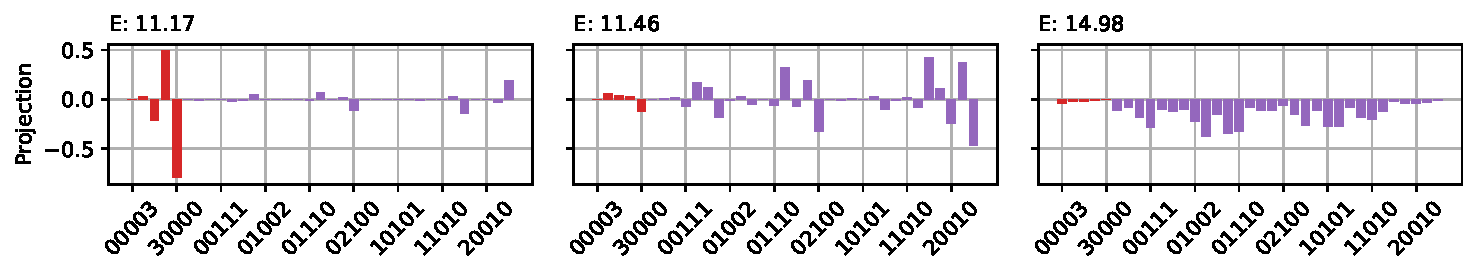
\includegraphics[width=.33\linewidth]{Pictures/eigenstates2}
	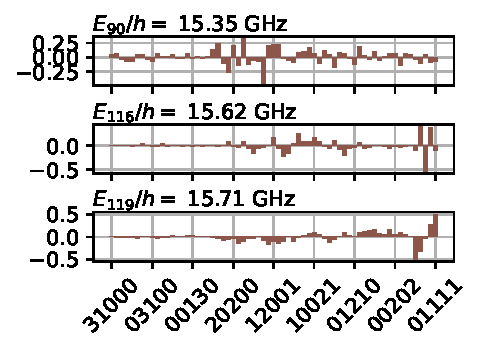
\includegraphics[width=.33\linewidth]{Pictures/eigenstates3}
	\caption{\textbf{(a)} The analytical solution for the $S_{21}$ in the linear regime (smooth curves) fitted to the low power data (clouds), normalized. \textbf{(b)} Experimental and simulated $S_{21}$ for various driving powers. Driving power is calibrated to match the Rabi frequency $\Omega$ of the simulation.  Dashes show the corresponding multi-photon transition frequencies calculated using the eigenlevels from (c).  \textbf{(c)} The energy level structure of the model with and without interaction using the parameters extracted from the fits; three excitations per site are included, and up to four excitations total; $E_n$ is the energy of the $n$-th eigenstate, $E_0 = 0$. \textbf{(d)} Relevant many-body eigenstates projected onto the unperturbed basis (colors as in (c)). The inherent randomness in the decompositions of the high-energy states conditions the random structure of the energy levels.}
	\label{fig:cq_transition}
\end{figure*}

The results of the DTS are shown in \autoref{fig:transmission}~(a). To show the structure of the eigenmodes and to extract $\omega_i$ and $J$, we bias one of the transmons across the degeneracy point while keeping the others at around 4.05 GHz. In the left column, the first transmon is swept, and in the right the middle one. The first transmon interacts with all collective modes, and the third only with the odd ones; this behavior is expected from the Hamiltonian. We find the tunnelling rate $J/2\pi$ to be around 41 MHz from the numerical fit. When the incident power is increased, the resonances are subject to photon blockade \cite{birnbaum2005photon} and behave similarly to what is observed for single superconducting qubits \cite{astafiev2010resonance}. In the bottom row of \autoref{fig:transmission}~(a), we notice spectral manifestations of the many-body states of the system which do not have any classical analogy and cannot be observed in a non-composite quantum system. We thus call this power-dependent behavior shown in \autoref{fig:transmission}~(a) the classical-quantum transition. 


The remaining parameters $\alpha_i$ of \autoref{eq:bose-hubbard} can be extracted via the CKS. In \autoref{fig:transmission}~(b) we have done it using the same two configurations of the transmon frequencies as in \autoref{fig:transmission}~(a) and performed another numerical fit (solid and dashed lines). The readout tone was aimed at the third mode, so the observed spectral frequencies should be corrected by adding its frequency for each bias voltage. The dashed lines show the emergent bands of the two-photon subspace: the many-body states with two excitations at different sites are near 4.05 GHz and ``doublons'' \cite{gorlach2018simulation} are located around 3.85 GHz. The Bose-Hubbard eigenstates with doubly-populated sites have lower energy due to the attractive interactions; the disorder in the extracted values of $\alpha_i/2\pi$ of approximately [-188, -178, -178, -178, -188] MHz is around 5\% and is caused by the uncompensated capacitance to the transmission lines. 
%\section{Classical to quantum transition}
%\begin{figure*}[t]
%	\centering
%	\caption{}
%	\label{fig:eigenstates}
%\end{figure*}

To further study the energy structure and the non-equilibrium dynamics of the system during the classical-quantum transition, we use a direct transmission experiment with fixed degenerate configuration of the transmon frequencies $\omega_i/2\pi = 3.9$ GHz. Using a fitting procedure similar to \autoref{fig:transmission} we find $\omega_i/2\pi$ to [3.898, 3.898, 3.9, 3.901, 3.901] MHz where differences from the target value come from the flux cross-talk. In the linear regime, we estimate the coupling to the transmission lines and internal dissipation from the fit of the complex transmission coefficient predicted by the linear model which is shown in \autoref{fig:cq_transition}~(a). Using these data, we also estimate the transmission amplitude through the attenuation and amplification chain and find that the third mode has nearly unity transmission. This is expected, as from \autoref{fig:transmission}~(a) it is only coupled to a single ``bulk'' transmon, and thus has the least internal dissipation. Since in the linear model it is impossible to discern pure dephasing and internal dissipation, the relaxation rates from the fit are larger than true values: we estimate $\gamma_i$ to be [16, 6, 0.1,  3, 16] $\mu\text{s}^{-1}$; the rates $\gamma_1$ and $\gamma_5$ are in good agreement with the value calculated from the simulated edge capacitances of 8 fF and justify the assumption of dominating $\Gamma$.

\autoref{fig:cq_transition}~(b) shows how the transmission spectrum changes throughout the transition. The normal mode peaks gradually saturate due to the photon blockage and the additional dips appear caused by the multiphoton transitions to the many-body eigenstates \cite{Biella2015,PhysRevA.102.013707,roberts2020driven}. The experimental data agrees very well with the numerical steady-state simulation in \textit{qutip} \cite{qutip1, qutip2} of the five-site Bose-Hubbard model with the parameters extracted earlier and three bosons per site at max; the simulation of 253$\times$253 density matrix takes approximately a week on a 138 core cluster for the shown 300$\times$300 heatmap. The selection rules of the system do not allow all possible multiphoton lines, but one can clearly discern an increase of the density of states and their randomness with increasing band number. It can be connected to the classical chaotisity of the system if the distribution of the level spacings corresponds to the Gaussian orthogonal ensemble \cite{bohigas1984characterization,zimmermann1986manifestation, livan2018introduction}. The frequencies of transitions up to four-photon are shown with colored dashes and can be identified with the energy bands shown in \autoref{fig:cq_transition}~(c) calculated using the fitted parameters of the model \autoref{eq:bose-hubbard}. We check that the statistics of the calculated nearest-neighbor level spacings resembles the Wigner-Dyson distribution for the experimentally determined parameters, but rather Poissonian for the ideal parameters which probably means that the system size is too low to obtain the correct histogram. To show how delocalized are the eigenstates $ \ket{E_n} $ reachable in our device, in \autoref{fig:cq_transition}~(d) we project several of them onto the non-interacting basis. State $\ket{E_1}$ has the structure identical to a classical symmetric low-frequency eigenmode. States $\ket{E_{11}}$ and $\ket{E_{20}}$ are at the edges of the orange band of the two-photon subspace and are much larger superpositions. One can note the unveiling randomness in the decomposition coefficients, which becomes more and more pronounced for higher energies: no symmetries or even any kind of structure can be found in the higher eigenstates except for the hole-like four-excitation subspace dual to the single-photon one (see $\ket{E_{116, 119}}$). 

\begin{figure}
	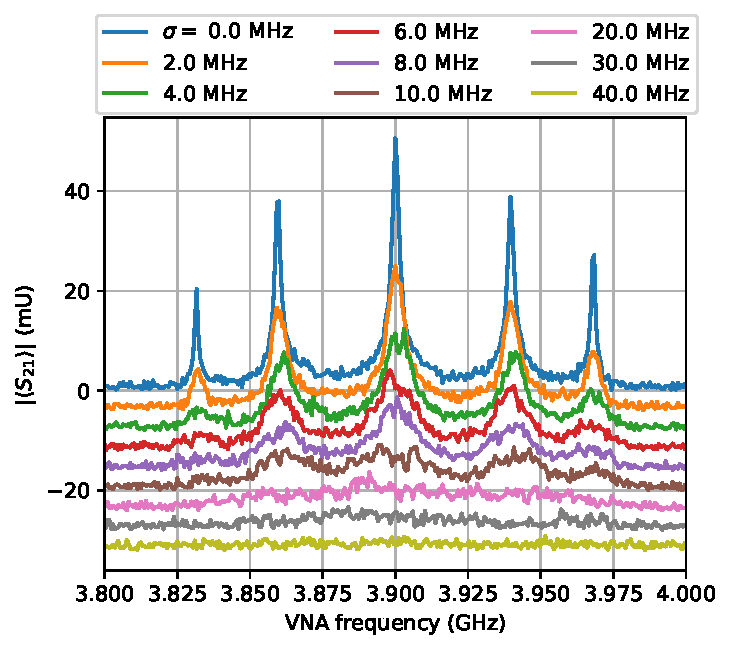
\includegraphics[width=1\linewidth]{Pictures/mbl}
	\caption{\textbf{(a)} Raw transmission data for $\sigma = 6,\, 40$ MHz and 100 realizations of disorder; absolute value of the transmission is shown with color. \textbf{(b)} Localization and disappearance of transmission with increasing disorder. Each curve shows the absolute value of the averaged transmission over the Gaussian disorder realizations with a certain standard deviation $\sigma$ shown in the legend. Each next curve is offset downwards for better visibility. \textbf{(c)} Probability distributions of the brightest peak prominence $\langle |S_{21}|^{max}\rangle$ (see text) observed in the disorder realizations for the $\sigma$ values from (b).}
	\label{fig:mbl}
\end{figure}

It is known that the Poissoinian statistics is usually a property of the disordered Bose-Hubbard model exhibiting localization \cite{roushan2017spectroscopic, Yan2019,Ye2019}. To check how the localization changes the transport properties, we introduce controllable disorder into the transmon frequencies near the degeneracy point in an experiment similar to what was done before numerically \cite{orell2019probing}: a certain common frequency variance $\sigma$ is chosen, then the random frequency $\omega + \delta \omega$ is assigned to each transmon where $\delta\omega \in \mathbb N(0,2\pi\sigma)$ and $\omega/2\pi = 3.9$ GHz. Then the transmission is recorded, and the full process is repeated 100 times. 
In \autoref{fig:mbl}~(a) we show two examples of the raw transmission data for  $\sigma = 6,\, 40$ MHz. As one can see, for the smaller standard deviation of the target frequencies, the eigenmodes stay relatively unchanged while for the larger the initial structure is completely lost. The averaged curves for several values of $\sigma$ are shown in \autoref{fig:mbl}~(b). One can see that when the noise in the transmon frequencies reaches the coupling strength $J/2\pi$, the averaged transmission vanishes. This means that the localization is revealed in the transport properties when the excitation of the first qubit on average does not reach the last qubit. This fact reminds of the superconductor-insulator transition \cite{bruder1993superconductor} to describe which was the initial purpose of the Bose-Hubbard model. As the transmission vanishes only on average and some peaks occasionally remain even for the largest $\sigma$, in \autoref{fig:mbl}~(c) we also study the distribution of the brightest peak prominences (taken as the mean of 10 points around the maximum) seen over the disorder realizations and show that is changes qualitatively when $\sigma \approx J/2\pi$.  

As we only study the lowest excited modes of the system in the linear regime, one can argue that this effect may be equally well described by the classical coupled mode theory. Similarly, the thermalization of a system of coupled linear oscillators would not occur when a single normal \textit{mode} is excited \cite{deutsch2018eigenstate}, but when a single \textit{oscillator} is, the behavior of such system should be identical to the one tested for chains of coupled transmons before \cite{Yan2019, ma2019dissipatively} for low disorder configurations and single-photon states; the observed values would then be not the populations of the single-transmon Fock-states but the amplitudes of the oscillations at each site. However, this is only a shallow analogy showing the continuity between classical and quantum physics \cite{park2012classical}.

In conclusion, we have shown how quantum photon transport occurs through a Bose-Hubbard chain modeled by a chain of five transmons. We have demonstrated that the behavior of the single-photon subspace of the system does not deviate from the classical normal mode theory which is expected from the correspondence principle. However, an increase of the incident photon flux beyond the dissipation rate reveals the quantum nature of the system through the photon blockade and multiphoton transitions to composite many-body states. The classical theory then fails, and one can only resort to numerical solution of the master equation to find the non-equilibrium steady state, which shows excellent agreement with the data. Finally, we have shown how controllable disorder affects the photon transport: we find that the transmission averaged over disorder realizations ceases when the standard deviation of the transmon frequencies reaches the interaction strength.

We gratefully acknowledge valuable discussions with I.S. Besedin and S. Flach. We thank E. Egorova, I. Tsitsilin and A. Sokolova for their help in designing the sample and preliminary experiments. We thank  A. A. Dobronosova, D. O. Moskalev, A. A. Pishchimova, E. I. Malevannaya for the fabrication of the device. The investigation was conducted with the support of Russian Science Foundation, Grants No. 16-12-00070 (measurement and data analysis) and 16-12-00095 (numerical modeling). Devices were fabricated at the BMSTU Nanofabrication Facility (Functional Micro/Nanosystems, FMNS REC, ID 74300). We also acknowledge support from the Ministry of Education and Science of the Russian Federation in the framework of the Increased Competitiveness Program of the National University of Science and Technology MISIS (Contract No. K2-2020-017). 


\bibliography{papers_bibliography}% Produces the bibliography via BibTeX.	
\end{document}